\documentclass[aspectratio=169,10pt]{beamer}
\usepackage[T1]{fontenc}
\usepackage{lmodern}
\usepackage{tikz}
\usetikzlibrary{arrows.meta,positioning}

\definecolor{BirdiNavy}{HTML}{173B63}
\definecolor{BirdiBlue}{HTML}{275A91}
\definecolor{BirdiTeal}{HTML}{238A83}
\definecolor{BirdiAlert}{HTML}{B64B43}
\definecolor{BirdiGreen}{HTML}{3E7D4A}
\definecolor{BirdiPanel}{HTML}{EAF1F8}
\definecolor{BirdiInk}{HTML}{202830}
\definecolor{BirdiMuted}{HTML}{607080}

\setbeamertemplate{navigation symbols}{}
\setbeamercolor{normal text}{fg=BirdiInk,bg=white}
\setbeamercolor{frametitle}{fg=white,bg=BirdiNavy}
\setbeamercolor{structure}{fg=BirdiBlue}
\setbeamerfont{frametitle}{size=\Large,series=\bfseries}
\setbeamertemplate{frametitle}{%
  \nointerlineskip
  \begin{beamercolorbox}[wd=\paperwidth,ht=.78cm,dp=.24cm,leftskip=.42cm]{frametitle}
    \insertframetitle
  \end{beamercolorbox}}
\setbeamertemplate{footline}{%
  \begin{beamercolorbox}[wd=\paperwidth,ht=.34cm,dp=.12cm,leftskip=.42cm,rightskip=.42cm]{frametitle}
    \scriptsize BIRDI research journey: graph latent $\rightarrow$ typed IR $\rightarrow$ verified RTL
    \hfill \insertframenumber/2
  \end{beamercolorbox}}

\newenvironment{stageblock}[2]{%
  \setbeamercolor{block title}{fg=white,bg=#1}%
  \setbeamercolor{block body}{fg=BirdiInk,bg=white}%
  \begin{block}{#2}\scriptsize}{\end{block}}

\begin{document}

\begin{frame}{Evolution of the BIRDI research pipeline}
\scriptsize\color{BirdiMuted}
From latent structural learning to explicit plans and executable verification.
\par\medskip

\begin{columns}[T,onlytextwidth]
\column{.32\textwidth}
\begin{stageblock}{BirdiBlue}{1. Graph-latent Python}
\textbf{Representation:} AST + state/data-flow graph latent.\par\medskip
\colorbox{BirdiPanel}{\parbox{.92\linewidth}{\ttfamily code graph $\to$ JEPA $\to$ graph decoder $\to$ Python}}\par\medskip
\textcolor{BirdiBlue}{\textbf{What we retained}}\par
Structural supervision and contrastive alignment organized problem and solution representations.\par\medskip
\textcolor{BirdiAlert}{\textbf{Why we evolved}}\par
The decoder drifted semantically; small prompt changes could produce the same incorrect logic.
\end{stageblock}

\column{.32\textwidth}
\begin{stageblock}{BirdiTeal}{2. Typed IR + retrieval}
\textbf{Representation:} compact typed algorithm DSL / IR.\par\medskip
\colorbox{BirdiPanel}{\parbox{.92\linewidth}{\ttfamily JEPA $\to$ top-$k$ IR $\to$ CodeT5+ repair $\to$ compiler}}\par\medskip
\textcolor{BirdiTeal}{\textbf{What we retained}}\par
An explicit target made retrieval, repair, and final compilation separately diagnosable.\par\medskip
\textcolor{BirdiAlert}{\textbf{Why we evolved}}\par
Algorithm composition remained limited when retrieval and repair data lacked the needed variation.
\end{stageblock}

\column{.32\textwidth}
\begin{stageblock}{BirdiGreen}{3. Verified RTL agents}
\textbf{Representation:} Verilog + executable oracle evidence.\par\medskip
\colorbox{BirdiPanel}{\parbox{.92\linewidth}{\ttfamily RTL $\to$ tests $\to$ Icarus $\to$ repair $\to$ benchmark}}\par\medskip
\textcolor{BirdiGreen}{\textbf{What we retained}}\par
Compilation, simulation, mismatch traces, and repair connect output to measurable behavior.\par\medskip
\textcolor{BirdiAlert}{\textbf{Remaining weakness}}\par
Random stimuli can miss rare states, and agents can agree on the same wrong behavior.
\end{stageblock}
\end{columns}

\vfill
\begin{beamercolorbox}[wd=\linewidth,sep=.65ex,center]{block body}
\textbf{Design principle:} latent graph $\rightarrow$ explicit typed IR $\rightarrow$ executable behavioral evidence
\end{beamercolorbox}
\end{frame}

\begin{frame}{Current implementation: verify and repair before final scoring}
\scriptsize\color{BirdiMuted}
The same RTL generator is evaluated under two oracle-family conditions; official VerilogEval is evaluation-only.
\par\smallskip

\begin{tikzpicture}[every node/.style={font=\scriptsize,align=center},
  step/.style={draw=BirdiMuted!45,fill=BirdiPanel,minimum height=.74cm,minimum width=2.15cm}]
\node[step] (s1) {RTL spec};
\node[step,right=.25cm of s1] (s2) {Qwen RTL\\generator};
\node[step,right=.25cm of s2] (s3) {Qwen/DeepSeek\\oracle package};
\node[step,right=.25cm of s3] (s4) {Icarus compile\\+ simulation};
\node[step,right=.25cm of s4] (s5) {Repair};
\node[step,right=.25cm of s5] (s6) {Official\\pass@1};
\foreach \a/\b in {s1/s2,s2/s3,s3/s4,s4/s5,s5/s6}
  \draw[-{Latex[length=1.8mm]},BirdiMuted] (\a)--(\b);
\end{tikzpicture}

\vspace{.3cm}
\begin{columns}[T,onlytextwidth]
\column{.48\textwidth}
\begin{stageblock}{BirdiBlue}{Preliminary VerilogEval pass@1}
50-task complexity-weighted subset.\par\medskip
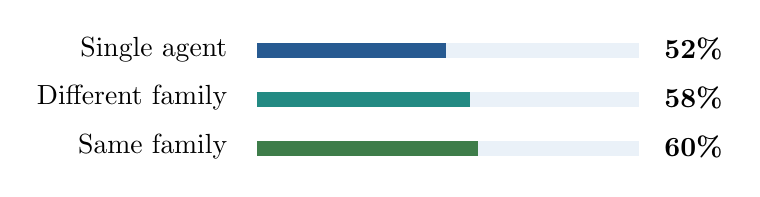
\begin{tikzpicture}[x=5.1cm,y=.62cm]
\node[anchor=east] at (0,2) {Single agent};
\fill[BirdiPanel] (.05,1.82) rectangle (1,2.12);
\fill[BirdiBlue] (.05,1.82) rectangle (.52,2.12);
\node[anchor=west,font=\bfseries] at (1.04,2) {52\%};
\node[anchor=east] at (0,1) {Different family};
\fill[BirdiPanel] (.05,.82) rectangle (1,1.12);
\fill[BirdiTeal] (.05,.82) rectangle (.58,1.12);
\node[anchor=west,font=\bfseries] at (1.04,1) {58\%};
\node[anchor=east] at (0,0) {Same family};
\fill[BirdiPanel] (.05,-.18) rectangle (1,.12);
\fill[BirdiGreen] (.05,-.18) rectangle (.60,.12);
\node[anchor=west,font=\bfseries] at (1.04,0) {60\%};
\end{tikzpicture}
\end{stageblock}

\column{.48\textwidth}
\begin{stageblock}{BirdiGreen}{Interpretation and next experiment}
\begin{enumerate}\scriptsize
  \item Both oracle + repair paths improved over the same generator.
  \item Same-family Qwen reached 60\%; different-family DeepSeek reached 58\%. Diversity was not automatically superior.
  \item Next, compare random-only verification against directed, metamorphic, coverage-guided, and bounded-formal checks.
\end{enumerate}
\end{stageblock}
\end{columns}
\end{frame}

\end{document}
